%#!pdfpLaTeX
%
% 北村研究室用卒論予稿のTeXテンプレートファイル
% 本ファイルは非公式であり,下記で公開されているワードのテンプレートが公式である.
% https://www.kagawa-nct.ac.jp/EE/local/index.html (学内限定アクセス)
%
% 2020年1月18日 北村大地作成
%

\documentclass[a4j]{jsarticle}
\usepackage{nitkagawaproc5ec} % 予稿テンプレートクラスファイル
\usepackage{amsmath,amssymb} % 数式環境
\usepackage{bm} % 数式の太字斜体
\usepackage[dvipdfmx]{color}
\usepackage[dvipdfmx]{graphicx}
\usepackage[caption=false]{subfig}
\usepackage{flushend} % 2段組みの最終ページの高さを揃える

\renewcommand{\baselinestretch}{0.8} % 行間設定(標準は0.8)
\newcommand{\red}[1]{\textcolor{black}{#1}}
\newcommand{\blue}[1]{\textcolor{blue}{\Sl{}}}

%%%%%%%%%%%%%%%%%%%%%%%%%%% 論文情報 %%%%%%%%%%%%%%%%%%%%%%%%%%%

%%%%% タイトル %%%%%
\title{深層パーミュテーション解決法の基礎的検討}
\etitle{Basic study for deep permutation solver}

%%%%% 著者 %%%%%
\author{蓮池 郁也}
\eauthor{Fumiya Hasuike}


%----- 図表題が英語の場合は次の2行を有効化 -----%
\renewcommand{\figurename}{Fig.~} 
\renewcommand{\tablename}{Table~}
%--------------------------------------------%

\begin{document}
\maketitle% タイトル生成

%----- ハイフン付きページ番号を表示する場合は次3行を有効化 -----%
%\setcounter{page}{1} % 開始ページ番号(3にすると3ページと4ページの2枚になる)
%\pagestyle{hyphenpage}
%\thispagestyle{hyphenpage}
%---------------------------------------------------------%

%----- ハイフン無しページ番号を表示する場合は次3行を有効化 -----%
%\setcounter{page}{1} % 開始ページ番号(3にすると3ページと4ページの2枚になる)
%\thispagestyle{plain}
%\pagestyle{plain}
%---------------------------------------------------------%

%----- ページ番号を削除する場合は次2行を有効化 -----%
\thispagestyle{empty}
\pagestyle{empty}
%-----------------------------------------------%

%%%%%%%%%%%%%%%%%%%%%%%%%%% 本文 %%%%%%%%%%%%%%%%%%%%%%%%%%%
%----------------------------------------------
\section{はじめに}
%----------------------------------------------
音源位置やマイクロフォン位置等が未知の条件で音源分離を達成する技術はブラインド音源分離(BSS)と呼ばれる.
観測信号のチャネル数(マイクロフォン数)と混合されている音源数が等しい条件下では,観測信号を時間周波数領域に変換し周波数毎に独立成分分析(ICA)\cite{ICA}を適用する時間周波数領域ICA(FDICA)\cite{FDICA}が提案されている.
ICAは一般に推定分離信号の順番が不定であり,FDICAはFig.~\ref{fig:permu}に示すように周波数毎に独立なICAによるBSSを行うため,分離信号の順番が周波数毎にばらばらになってしまう問題が生じる.
この問題は一般に「パーミュテーション問題」と呼ばれている.
過去様々な解決法が提案されたが,あらゆる音源に適用可能な手法は未だ存在しない.

本稿では,様々な音源に適用可能なパーミュテーション解決法の構築を目的として,DNNの活用を検討する.
また,提案する深層パーミュテーション解決法を音声及び音楽信号に適用し,深層パーミュテーション解決法の実現可能性を調査する.

%----------------------------------------------
\section{FDICAとパーミュテーション問題}
%----------------------------------------------
ICAは音源間の統計的独立性のみに基づいて分離行列を推定するため,周波数毎に独立なICAを適用しているFDICAで推定される分離信号
\begin{align}
\bm{y}_{ij} &= \hat{\bm{W}}_i\bm{x}_{ij} \label{eq:sepSig}
\end{align}
はFig.~\ref{fig:permu}に示すように,推定音源の順番が周波数毎にばらばらになっている状態である.
ここで,$i = 1,2, \cdots, I$及び$j = 1,2, \cdots, J$はそれぞれ周波数及び時間のインデクス,$\bm{y}_{ij}$,$\bm{x}_{ij}$,及び$\bm{W}_{i}$はそれぞれ分離信号,観測信号,及び分離行列を示す.
またFig. 1に示すように,音源信号,観測信号,FDICAの推定信号,及びパーミュテーション問題解決後の信号の各時間周波数行列をそれぞれ$\bm{S}_n\in\mathbb{C}^{I\times J}$,$\bm{X}_m\in\mathbb{C}^{I\times J}$,
$\bm{Y}_n\in\mathbb{C}^{I\times J}$,及び$\bm{Z}_n\in\mathbb{C}^{I\times J}$と定義する($n=1, 2, \cdots, N$及び$m=1, 2, \cdots, M$はそれぞれ音源及びマイクロホンのインデクス).
FDICAで得られる$\bm{Y}_n$は,周波数毎の音源分離はできており,周波数間の推定音源の順序が統一されていない状態である.
これがパーミュテーション問題であり,全周波数の推定音源が同じ順序となるよう並び替える処理が必要となる.
%%%%%%%%%%%%%%%%%%%%%%%%%%%%
\begin{figure}[t]
  \vspace{15pt}
  \begin{center}
      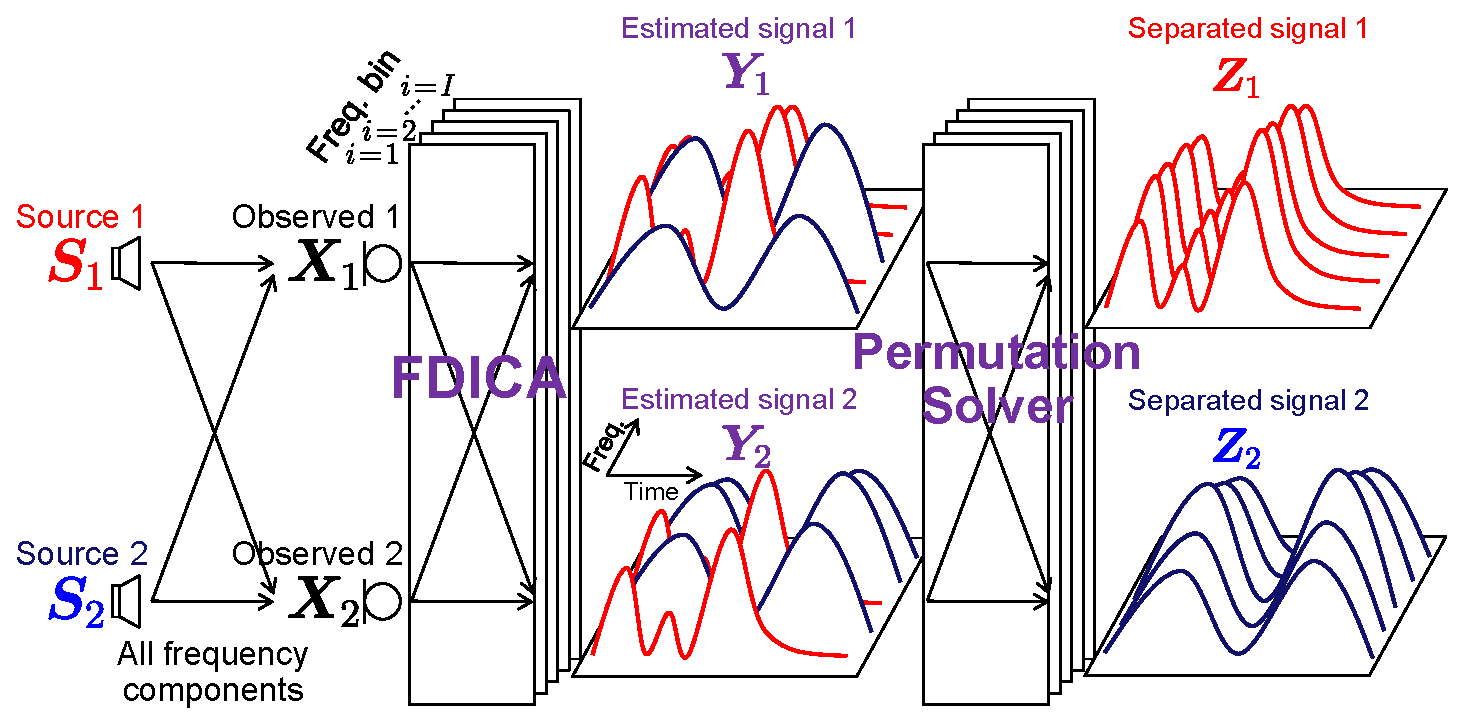
\includegraphics[width=1.0\columnwidth]{figures/permutation_image.eps}
  \end{center}
  \vspace{-8pt}
\caption{Permutation problem in FDICA.}
\label{fig:permu}
\end{figure}
%%%%%%%%%%%%%%%%%%%%%%%%%%%%
%----------------------------------------------
\section{提案手法}
%----------------------------------------------
%----------------------------------------------
\subsection{DNNの入出力}
%----------------------------------------------
%%%%%%%%%%%%%%%%%%%%%%%%%%%%
\begin{figure}[t]
  \begin{center}
      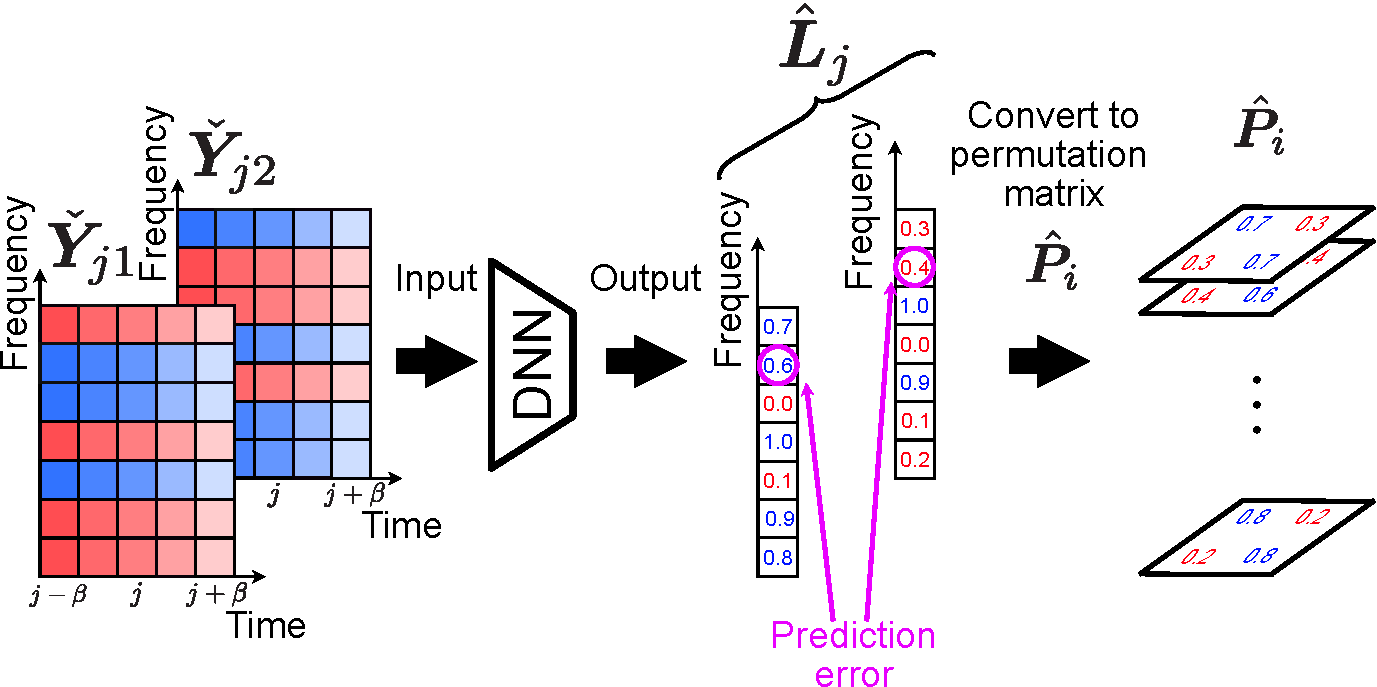
\includegraphics[width=1.00\columnwidth]{figures/cal_loss1.pdf}
  \end{center}
  \vspace{-8pt}
\caption{Calculatation of predicted permutation matrix.}
\label{fig:cal_loss1}
\vspace{-18pt}
\end{figure}
%%%%%%%%%%%%%%%%%%%%%%%%%%%%
%%%%%%%%%%%%%%%%%%%%%%%%%%%%
\begin{figure*}[t]
  \begin{center}
      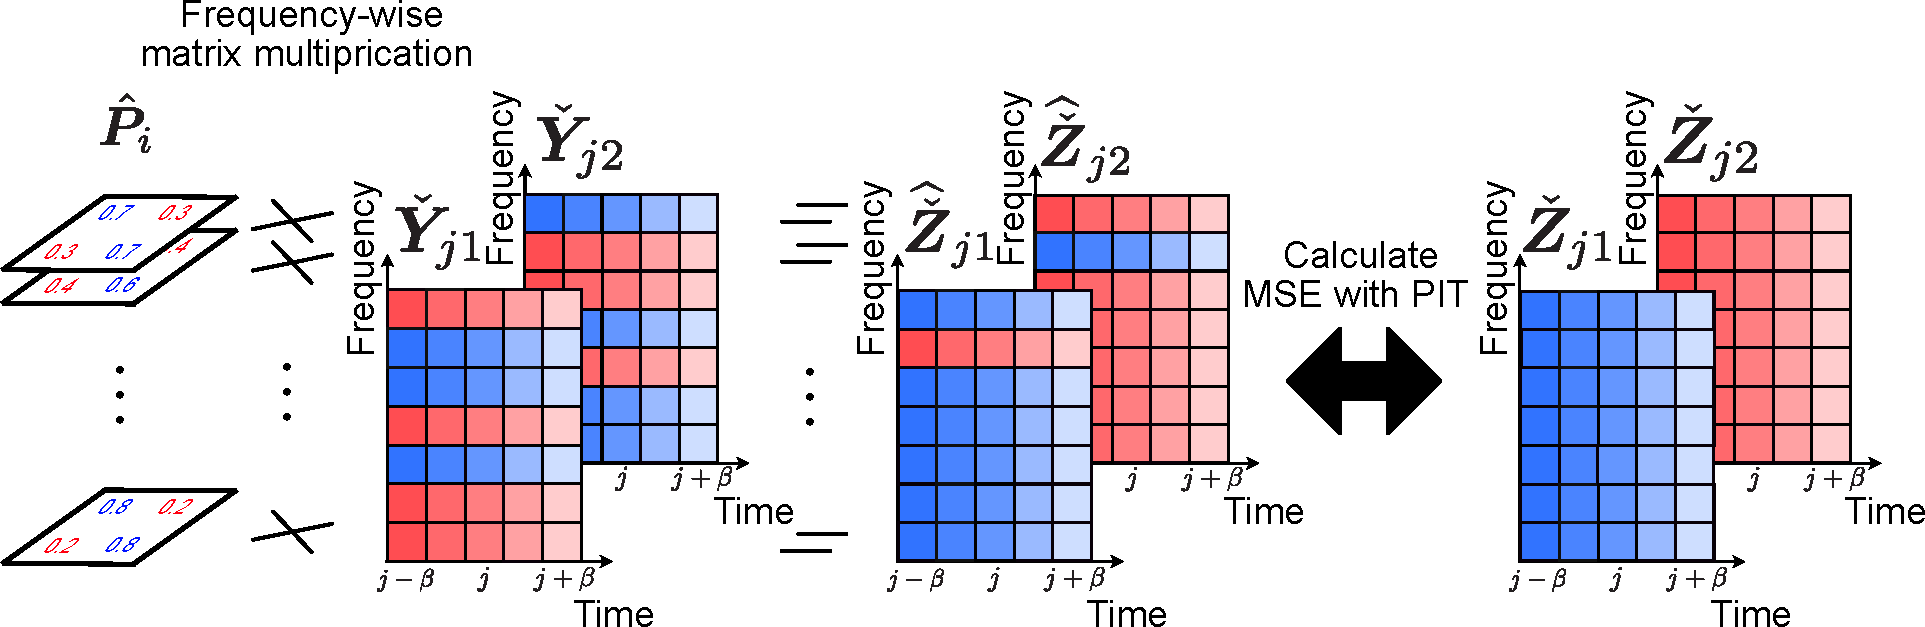
\includegraphics[width=2.0\columnwidth]{figures/cal_loss2.pdf}
  \end{center}
  \vspace{-8pt}
\caption{Calculation of MSE with PIT.}
\label{fig:cal_loss2}
\end{figure*}
%%%%%%%%%%%%%%%%%%%%%%%%%%%%
本稿では$N=M=2$の状況のみを取り扱う.
DNNの入力の前処理として,FDICAの推定信号$(\bm{Y}_1, \bm{Y}_2)$にパワー比の正規化\cite{Permutation_solverBSS}と時間フレーム$j$近傍のスペクトルの抽出を施す.
この前処理を適用した後の信号を$(\check{\bm{Y}}_{j1}, \check{\bm{Y}}_{j2})$と定義し,これらをベクトル化しDNNに入力する.
DNNの出力は周波数毎の確率値$(\hat{l}_{i1j}, \hat{l}_{i2j})$であり.$\hat{l}_{i1j}+\hat{l}_{i2j}=1$を満たす.
この$\hat{l}_{inj}$は入力の各周波数成分が$n$番目の音源の成分である確率を表しており,2音源であれば次式のようにパーミュテーション行列$\hat{\bm{P}}_i$に変換できる.
\begin{align}
  \hat{\bm{P}}_i = 
  \begin{bmatrix}
    \hat{l}_{i1j} & \hat{l}_{i2j} \\
    \hat{l}_{i2j} & \hat{l}_{i1j}
  \end{bmatrix} \label{eq:permMat}
\end{align}
上記の処理をFig.~\ref{fig:cal_loss1}に示す.
このとき,パーミュテーション問題は次式で解決される.
\begin{align}
  \hat{\bm{z}}_{ij} = \hat{\bm{P}}_i \bm{y}_{ij} \label{eq:reconstruct}
\end{align}
なお,式\eqref{eq:reconstruct}で得られる予測分離信号の時間周波数行列を$(\hat{\bm{Z}}_1, \hat{\bm{Z}}_2)$と定義する.
%----------------------------------------------
\subsection{DNNの構造と損失関数}
%----------------------------------------------
提案手法で用いるDNNの構造は,入力層,隠れ層3層,及び出力層の計5層の全結合層からなる多層パーセプトロンである.
また損失関数は,$\hat{\bm{P}}_i$に従って$(\check{\bm{Y}}_{j1}, \check{\bm{Y}}_{j2})$を並び替えた局所時間分離信号$(\check{\bm{Z}}_{j1}, \check{\bm{Z}}_{j2})$と
局所時間予測分離信号$(\widehat{\check{\bm{Z}}}_{j1}, \widehat{\check{\bm{Z}}}_{j2})$間の平均二乗誤差を順序不変学習(PIT)\cite{PIT}として定義している.
この一連の流れをFig.~\ref{fig:cal_loss2}に示す.
DNNはこの処理により得た損失値を用いて誤差逆伝播を行い,最適なモデルを学習する.
%----------------------------------------------
\section{実験}
%----------------------------------------------

%----------------------------------------------
\subsection{実験条件}
%----------------------------------------------
本稿では,実際の音声及び音楽信号の時間周波数行列にパーミュテーション問題を起こし,提案手法でどの程度解決できるか調査した.
このとき,学習データとして300パターンのパーミュテーション問題を生じさせた$(\bm{Y}_1, \bm{Y}_2)$を用意し,検証及びテストデータは学習データに含まれないパーミュテーション問題を用いた.
音声及び音楽信号はそれぞれ男女の英語発話及びドラムとピアノの音楽を用いた.
パーミュテーション問題の解決性能は信号対歪み比(SDR)の改善量で評価する.
SDRとは,音源分離の度合と分離音の歪みの少なさの両方を加味した客観評価尺度である.

%----------------------------------------------
\subsection{実験結果}
%----------------------------------------------

Fig.~\ref{fig:audio_16block}は実際の男女の音声信号に対するパーミュテーション問題が生じているスペクトログラム$(\bm{Y}_1, \bm{Y}_2)$及び予測結果$(\hat{\bm{Z}}_1, \hat{\bm{Z}}_2)$を示している.
$(\bm{Y}_1, \bm{Y}_2)$は,各周波数毎に男女の信号が混ざっており一貫性のないスペクトログラムとなっているが,$(\hat{\bm{Z}}_1, \hat{\bm{Z}}_2)$は,
各周波数成分に連続性が見られる.
即ち,男女のどちらの信号も高い精度でスペクトログラムを予測できていることが分かる.
DNNの学習データ及び検証データに対する正答率は90\%を超えており,ほとんどの周波数成分を正しく並び替えできていることが分かる.
SDRの改善量は,$(\hat{\bm{Z}}_1,\hat{\bm{Z}}_2)$に対してそれぞれ26.7~dB,及び31.0~dBであり,提案手法による分離精度が高いことを示している.

%%%%%%%%%%%%%%%%%%%%%%%%%%%%
\begin{figure}[t]
  \begin{center}
      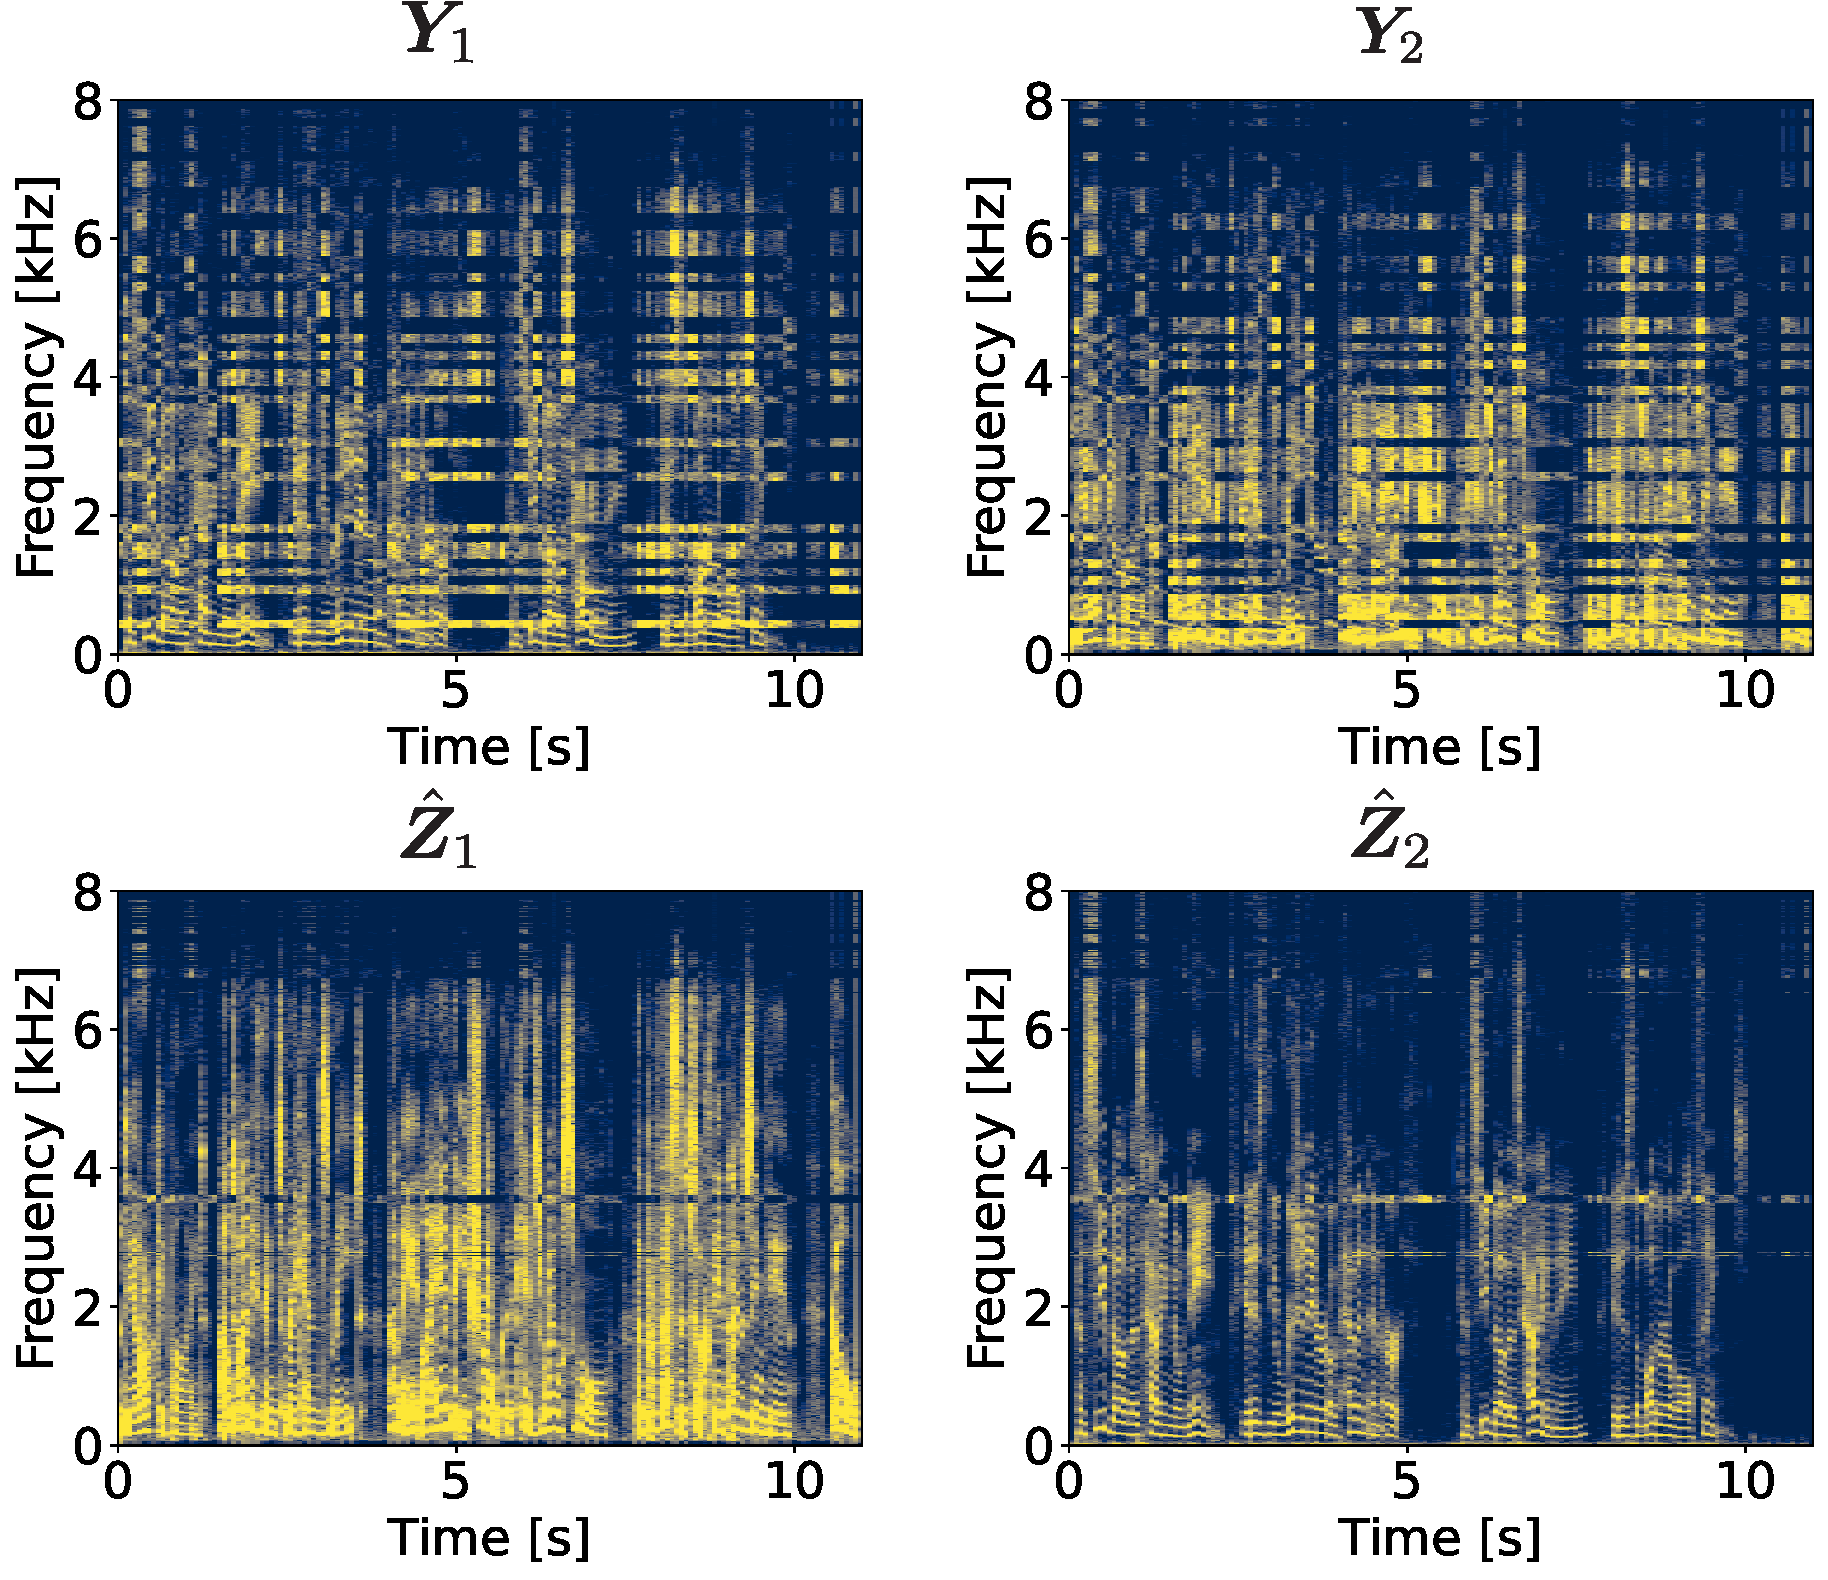
\includegraphics[width=1.0\columnwidth]{figures/audio_16block.pdf}
  \end{center}
  \vspace{-15pt}
\caption{Input spectrograms with permutation problem (upper) and permutation-aligned spectrograms using predicted results (bottom).}
\label{fig:audio_16block}
\vspace{-15pt}
\end{figure}
%%%%%%%%%%%%%%%%%%%%%%%%%%%%
%----------------------------------------------
\section{まとめ}
%----------------------------------------------
本稿では,FDICAに伴うパーミュテーション問題の解決を目的とし,深層パーミュテーション解決法を新たに提案した.
実験結果より,DNNはパーミュテーション問題の解決に有効である可能性が示唆された.

%%%%% 参考文献 %%%%%
\begin{thebibliography}{9}% 10以上の文献数であれば99とする
%参考文献のフォントサイズを小さくしたい場合は下記2行のコメントアウトを解除
%\itemsep 3pt % 項目の間隔微調整用
%\fontsize{8pt}{10pt}\selectfont  % 項目のフォントサイズ微調整用
\scriptsize{
\bibitem{ICA}
P.~Comon, ``Independent component analysis, a new concept?,'' \textit{Signal Processing}, vol. 36, no. 3, pp. 287--314, 1994.

\bibitem{FDICA}
P.~Smaragdis, ``Blind separation of convolved mixtures in the frequency domain,'' \textit{Neurocomputing}, vol. 22, pp. 21--34, 1998.

\bibitem{Permutation_solverBSS}
H. Sawada, S. Araki, and S. Makino, ``Measuring dependence of bin-wise separated signals for permutation alignment in frequency-domain BSS,'' \textit{Proc. IEEE International Symposium on Circuits and Systems}, pp. 3247--3250, 2007.

\bibitem{PIT}
D. Yu, M. Kolbak, Z.-H. Tan, and J. Jensen, ``Permutation invariant training of deep models for speaker-independent multi-talker speech separation,'' \textit{Proc. IEEE International Conference on Acoustics, Speech and Signal Processing}, pp. 241-245, 2017. 
}
\end{thebibliography}

\end{document}